\documentclass{article}

\usepackage[a4paper, left=0.5in, right=0.5in, top=0.5in, bottom=0.5in]{geometry}
\usepackage{hyperref}
\usepackage{enumitem}
\usepackage{amsmath}
\usepackage{amssymb}
\usepackage{graphicx}
\usepackage{commath}
\usepackage{xcolor}
\usepackage{float}
\usepackage{minted}


\title{Divsion}
\author{Narendiran S}
\date{19-06-2021}

\begin{document}
\large
\maketitle

\section{Normal Divsion}
Division is a process of repeated subtraction.
If the Remainder is represented as R, the Divisor D and the Quotient Q.
Let the i'th digit of the Quotient be $q_i$.
So Q can be $\{ q_(n-1), q_(n-1), \dots, q_2, q_1, q_0 \}$.
If R(0) is the final Remainder, then ther general process of division can be expressed as,

\begin{align*}
    R(i) = R(i + 1) - q_i * D * 10^i
\end{align*}

Let's look at an examaple of 3148/3.
The steps of division can be seen below:

\begin{align*}
    3148 - 1 * 3 * 10^3 & =148  & \implies R(4) - q_3 * D * 10^3 & = R(3) \\
    148 - 0 * 3 * 10^2  & = 148 & \implies R(3) - q_2 * D * 10^2 & = R(2) \\
    148 - 4 * 3 * 10^1  & = 28  & \implies R(2) - q_1 * D * 10^1 & = R(1) \\
    28 - 9 * 3 * 10^0   & = 1   & \implies R(1) - q_0 * D * 10^0 & = R(0) \\
\end{align*}

\section{Restoring Division}

Source: \href{https://web.stanford.edu/class/ee486/doc/chap5.pdf}{web.stanford.edu}

Let's look into how to perform restroing division in decimal.

\begin{align*}
    q_3 = 1                  & \rightarrow R(3) = & 3148 - 3 * 10^3  & = +148                                   \\
    q_3 = 2                  & \rightarrow R(3) = & 148 - 3 * 10^3   & = -2852 \text{ (not positive - restore)} \\
    \textcolor{red}{q_3 = 1} & \rightarrow R(3) = & -2852 + 3 * 10^3 & = +148 \text{ (move on)}                 \\
    \\
    q_2 = 1                  & \rightarrow R(2) = & 148 - 3 * 10^2   & = -152 \text{ (not positive - restore)}  \\
    \textcolor{red}{q_2 = 0} & \rightarrow R(2) = & -152 + 3 * 10^2  & = +148 \text{ (move on)}                 \\
    \\
\end{align*}
\begin{align*}
    q_1 = 1                  & \rightarrow R(1) = & 148 - 3 * 10^1 & = +118                                \\
    q_1 = 2                  & \rightarrow R(1) = & 118 - 3 * 10^1 & = +88                                 \\
    q_1 = 3                  & \rightarrow R(1) = & 88 - 3 * 10^1  & = +58                                 \\
    q_1 = 4                  & \rightarrow R(1) = & 58 - 3 * 10^1  & = +28                                 \\
    q_1 = 5                  & \rightarrow R(1) = & 28 - 3 * 10^1  & = -2 \text{ (not positive - restore)} \\
    \textcolor{red}{q_1 = 4} & \rightarrow R(1) = & -2 + 3 * 10^1  & = +28 \text{ (move on)}               \\
\end{align*}
\begin{align*}
    q_0 = 1                  & \rightarrow R(0) = & 28 - 3 * 10^0 & = +25                                 \\
    q_0 = 2                  & \rightarrow R(0) = & 25 - 3 * 10^0 & = +22                                 \\
    q_0 = 3                  & \rightarrow R(0) = & 22 - 3 * 10^0 & = +19                                 \\
    q_0 = 4                  & \rightarrow R(0) = & 19 - 3 * 10^0 & = +16                                 \\
    q_0 = 5                  & \rightarrow R(0) = & 16 - 3 * 10^0 & = +13                                 \\
    q_0 = 6                  & \rightarrow R(0) = & 13 - 3 * 10^0 & = +10                                 \\
    q_0 = 7                  & \rightarrow R(0) = & 10 - 3 * 10^0 & = +7                                  \\
    q_0 = 8                  & \rightarrow R(0) = & 7 - 3 * 10^0  & = +4                                  \\
    q_0 = 9                  & \rightarrow R(0) = & 4 - 3 * 10^0  & = +1                                  \\
    q_0 = 10                 & \rightarrow R(0) = & 1 - 3 * 10^0  & = -2 \text{ (not positive - restore)} \\
    \textcolor{red}{q_0 = 9} & \rightarrow R(0) = & -1 + 3 * 10^0 & = +1 \text{ (move on)}                \\
\end{align*}

Applying this to binary by considering $q_i$'s to be set $\{0, 1\}$.
Now, the equation can be written as:

\begin{align*}
    R(i) = R(i + 1) - q_i * D * 2^i
\end{align*}

If $R(i) \ge 0$, then assuming $q_i = 1$ was correct.
If $R(i) < 0$, then assuming $q_i = 1$ was wrong, hence $q_i$ should be 0 and restoration must be done.

Let's perform a divison of 67/5.
The steps of division can be seen below:
\begin{align*}
    q_4 = 1                  & \rightarrow R(4) = & 67 - 5 * 2^4  & = -13 \text{ (not positive - restore)} \\
    \textcolor{red}{q_4 = 0} & \rightarrow R(4) = & -13 + 5 * 2^4 & = +67 \text{ (move on)}                \\
    \\
    \textcolor{red}{q_3 = 1} & \rightarrow R(3) = & 67 - 5 * 2^3  & = +27 \text{ (move on)}                \\
    \textcolor{red}{q_2 = 1} & \rightarrow R(2) = & 27 - 5 * 2^2  & = +7 \text{ (move on)}                 \\
    q_1 = 1                  & \rightarrow R(1) = & 7 - 5 * 2^1   & = -3 \text{ (not positive - restore)}  \\
    \textcolor{red}{q_1 = 0} & \rightarrow R(1) = & -3 + 5 * 2^1  & = +7 \text{ (move on)}                 \\
    \\
    \textcolor{red}{q_0 = 1} & \rightarrow R(0) = & 7 - 5 * 2^0   & = +2 \text{ (move on)}                 \\
\end{align*}

\subsection{Algorithm to Follow}
Assuming N bit's of input.

\begin{enumerate}
    \item Initlialize R with N bit zeros.
    \item Initlialize Q with N bit Dividend.
    \item Initlialize count with N.
    \item Combine R and Q to form a 2N bit register nameley \{R,Q\}.
    \item Perform the below operations till the count becomes zeros.
          \begin{itemize}
              \item Shift \{R,Q\} left by 1.
              \item Subtract M from R. (add 2's complement of M to R).
              \item If \verb|sign(R)| == 1
                    \begin{itemize}
                        \item Restore R with it's previous value. (Add M to R).
                        \item Set Q[0] = 0
                    \end{itemize}
              \item Else
                    \begin{itemize}
                        \item Set Q[0] = 1
                    \end{itemize}
              \item Decrement count by 1.
          \end{itemize}
    \item Finally, R gives the remainder and Q gives the Quotient.
\end{enumerate}

\subsection{Flow Chart}
\begin{figure}[H]
    \centering
    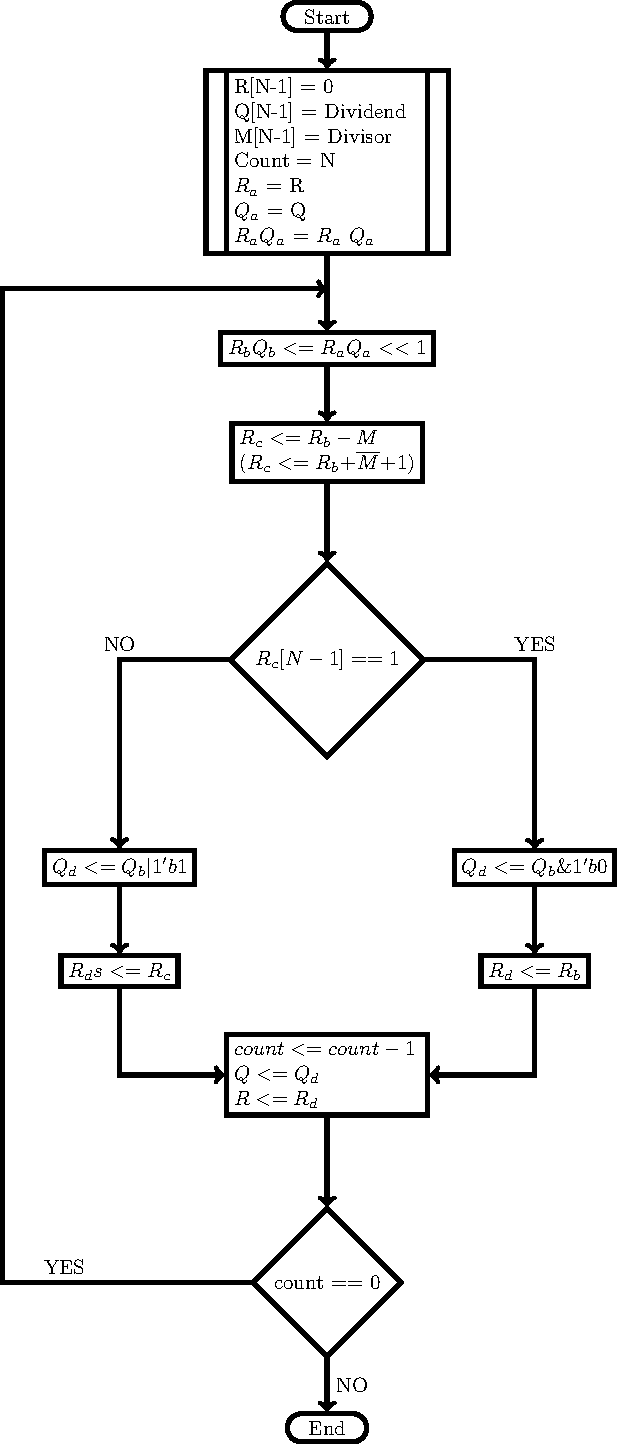
\includegraphics[scale=0.9]{../Resources/TexFiles/RestoringDivision.pdf}
\end{figure}

\subsection{Signed Division}
Signed Division can be done by converting to unsigned and based on the sign value we add sign to Quotient.

\begin{itemize}
    \item Find verb|sign = Dividend[N-1] xor Divisor[N-1]|.
    \item If Dividend[N-1] == 1, then Dividend is negative, convert to positive by performing two's complement.
    \item If Divisor[N-1] == 1, then Divisor is negative, convert to positive by performing two's complement.
    \item Finally, after division, if the sign is 1, then change the sign bit of Quotient to 1.    
\end{itemize}

\section{Non-Restoring Division}
Here, there is no Restoring done.
This is done by checking if the remainder is positive or negative and then Subtract. (which differs from restoring where subtraction is done and then checked)



Let's look into the binary divison of 67/3 using non-resoring division.
The steps of division can be seen below:
\begin{align*}
    q_4 = 1                  & \rightarrow R(4) = & 67 - 5 * 2^4  & = -13 \text{ (not positive)} \\
    \textcolor{red}{q_4 = 0}                                                                     \\
    \textcolor{red}{q_3 = 1} & \rightarrow R(3) = & -13 + 5 * 2^3 & = 27                         \\
    \textcolor{red}{q_2 = 1} & \rightarrow R(2) = & 27 - 5 * 2^2  & = 7                          \\
    q_1= 1                   & \rightarrow R(1) = & 7 - 5 * 2^1   & = -3 \text{ (not positive)}  \\
    \textcolor{red}{q_1 = 0}                                                                     \\
    \textcolor{red}{q_0 = 1} & \rightarrow R(0) = & -3 + 5 * 2^0  & = 2                          \\
\end{align*}



\subsection{Algorithm to Follow}
Assuming N bit's of input.

\begin{enumerate}
    \item Initlialize R with N bit zeros.
    \item Initlialize Q with N bit Dividend.
    \item Initlialize count with N.
    \item Combine R and Q to form a 2N bit register nameley \{R,Q\}.
    \item Perform the below operations till the count becomes zeros.
          \begin{itemize}
              \item If \verb|sign(R)| == 1
                    \begin{itemize}
                        \item Shift \{R,Q\} left by 1.
                        \item Add M to R.
                    \end{itemize}
              \item Else
                    \begin{itemize}
                        \item Shift \{R,Q\} left by 1.
                        \item Subtract M from R. (add 2's complement of M to R).
                    \end{itemize}
              \item If \verb|sign(R)| == 1
                    \begin{itemize}
                        \item Set Q[0] = 0
                    \end{itemize}
              \item Else
                    \begin{itemize}
                        \item Set Q[0] = 1
                    \end{itemize}
              \item Decrement count by 1.
          \end{itemize}
    \item If \verb|sign(R)| == 1
          \begin{itemize}
              \item Add M to R.
          \end{itemize}
    \item Finally, R gives the remainder and Q gives the Quotient.
\end{enumerate}

\subsection{Flow Chart}
\begin{figure}[H]
    \centering
    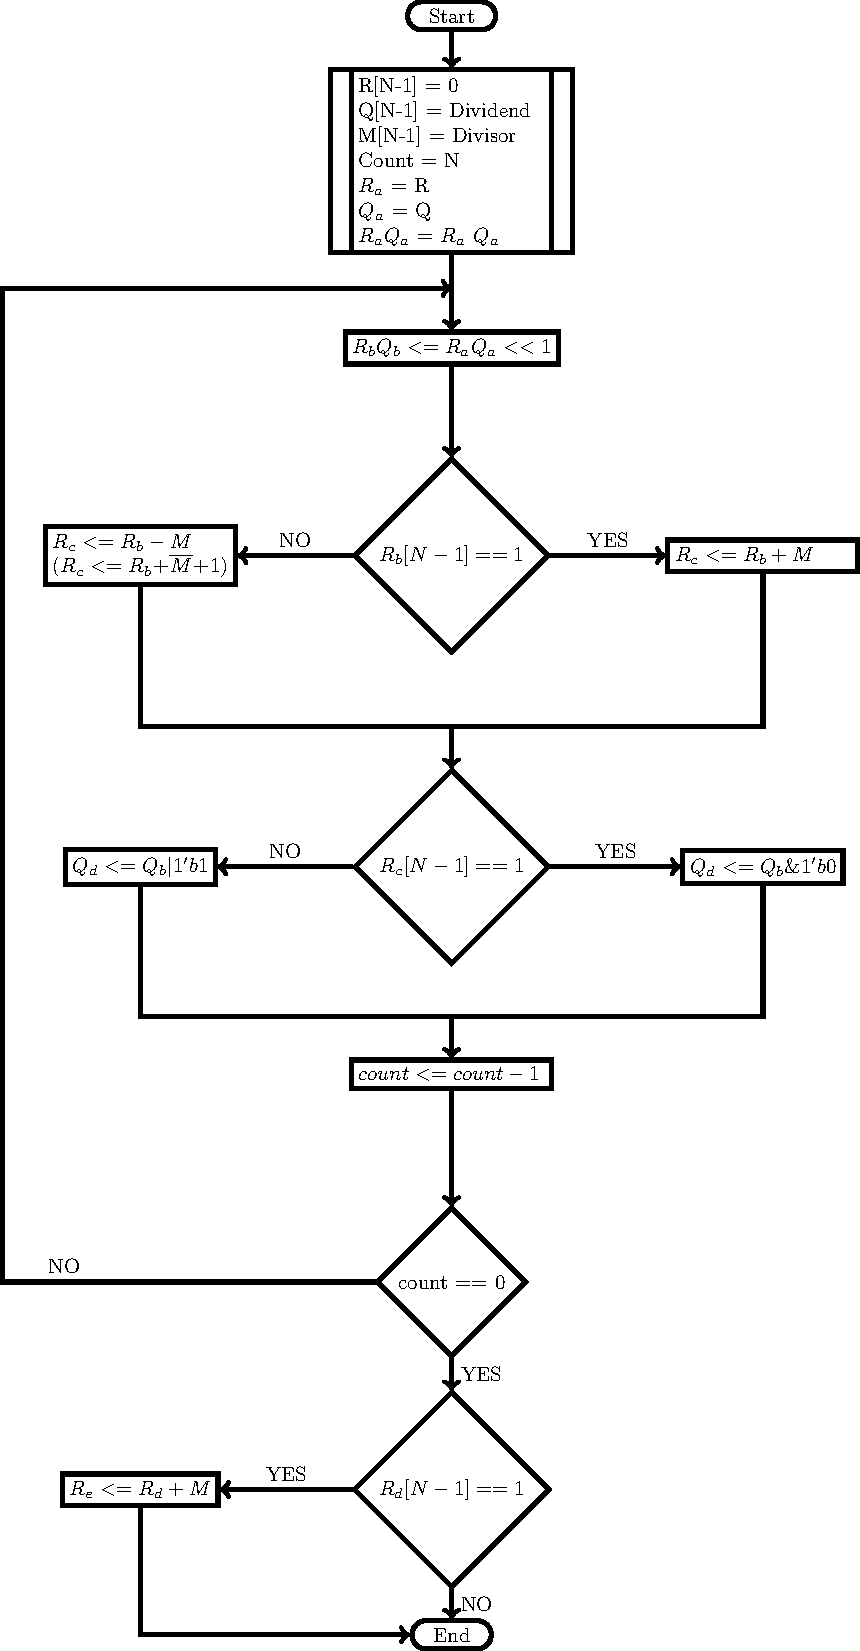
\includegraphics[scale=0.9]{../Resources/TexFiles/NonRestoringDivision.pdf}
\end{figure}

\subsection{Signed Division}
Signed Division can be done by converting to unsigned and based on the sign value we add sign to Quotient.

\begin{itemize}
    \item Find verb|sign = Dividend[N-1] xor Divisor[N-1]|.
    \item If Dividend[N-1] == 1, then Dividend is negative, convert to positive by performing two's complement.
    \item If Divisor[N-1] == 1, then Divisor is negative, convert to positive by performing two's complement.
    \item Finally, after division, if the sign is 1, then change the sign bit of Quotient to 1.    
\end{itemize}

\end{document}